\subsection{Desarrollo}
\label{subsec:desarrollo}

\subsubsection{Materiales e Instrumentos}

A continuación se detallan los materiales utilizados en cada práctica:

\begin{table}[H]
    \centering
    \label{tab:instrumentos}
    \begin{tabular}{|l|c|l|}
        \hline
        \textbf{Instrumento} & \textbf{Incertidumbre} & \textbf{Uso en la práctica} \\ \hline
        \csvreader[
            separator=semicolon,
            head=true,
            late after line=\\ \hline
        ]{secciones/desarrollo/instrumentos.csv}{}
        {\csvcoli & \csvcolii & \csvcoliii}
    \end{tabular}
\end{table}

\subsubsection{Procedimiento}

\paragraph{Práctica 1 --- Densidad del cilindro}
Se midió la altura $h$ y el diámetro $d$ del cilindro seis veces con cada instrumento (calibre y regla), anotando cada medición individualmente.
Con la probeta se realizó una sola medición de volumen por desplazamiento de agua, se anotó el nivel inicial, se introdujo el cilindro, y se registró el nivel final.
La masa se midió una sola vez con la balanza electrónica.

\begin{figure}[H]
    \centering
    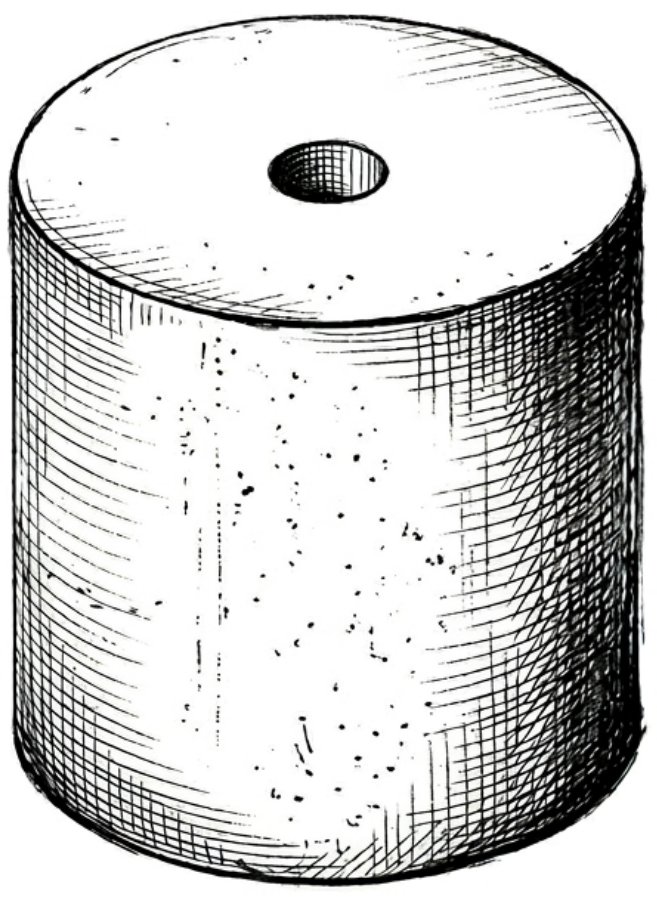
\includegraphics[width=0.15\textwidth]{secciones/desarrollo/esquema-cilindro}
    \caption{Dibujo esquemático del cilindro utilizado en la práctica.}
    \label{fig:diagrama-cilindro}
\end{figure}

\paragraph{Práctica 2 --- Péndulo ideal}
Se confeccionó un péndulo simple con una esfera colgada de un hilo.
Se midieron 4 longitudes distintas del hilo ($L$ = $1000$, $820$, $730$ y $517$ $mm$) con regla milimetrada.
Para cada longitud se registró el tiempo de 20 oscilaciones ($n = 20$) en 4 amplitudes distintas ($\theta = 5^{\circ}$, $9^{\circ}$, $15^{\circ}$ y $20^{\circ}$).
En algunos casos se realizaron dos mediciones del tiempo y se tomó el promedio.
Se utilizó $n = 20$ para reducir el error relativo en la medición del periodo $\Delta T = \frac{\Delta t}{n}$, ya que la incerteza de lectura del cronómetro (principalmente el error de reacción humana, $\sim$0,1--0,2 s) se distribuye sobre un intervalo de tiempo mayor.

\begin{figure}[H]
    \centering
    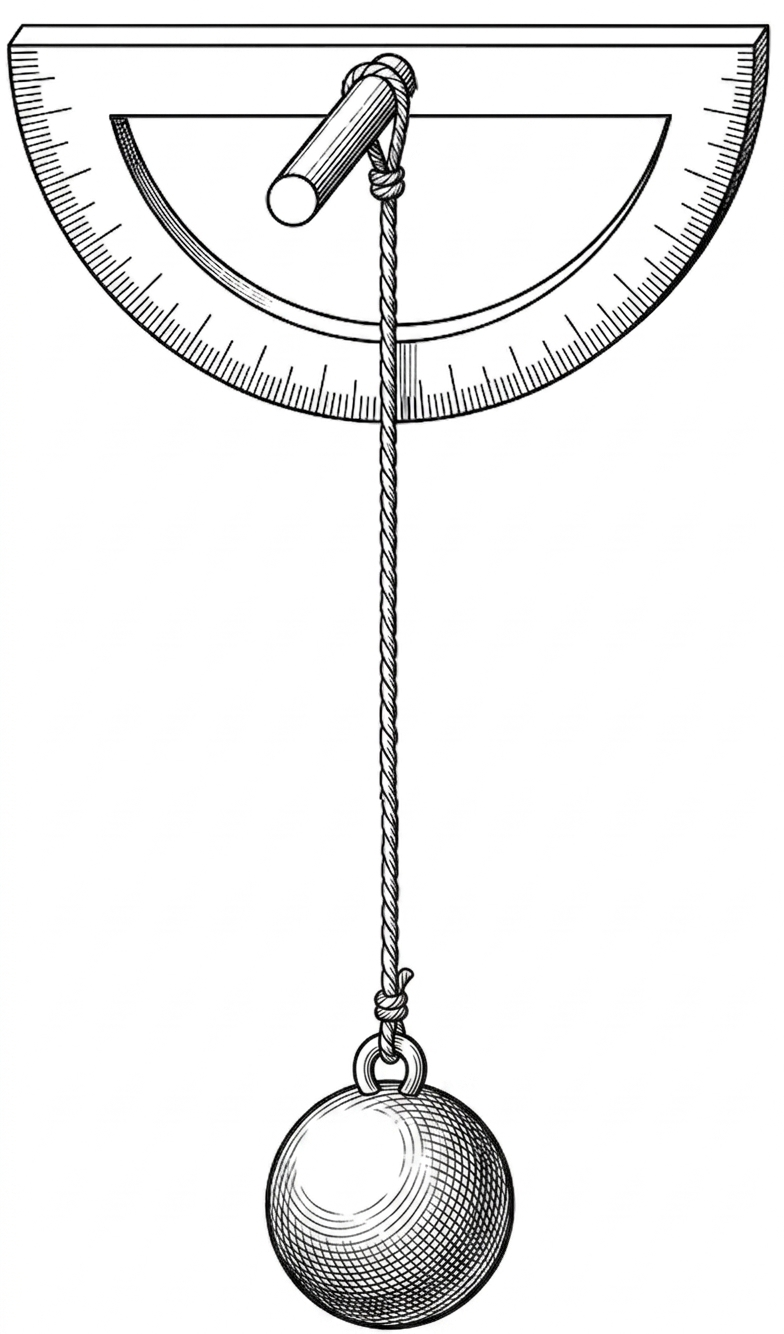
\includegraphics[width=0.3\textwidth]{secciones/desarrollo/esquema-pendulo}
    \caption{Dibujo esquemático del pendulo confeccionado en la práctica.}
    \label{fig:diagrama-pendulo}
\end{figure}